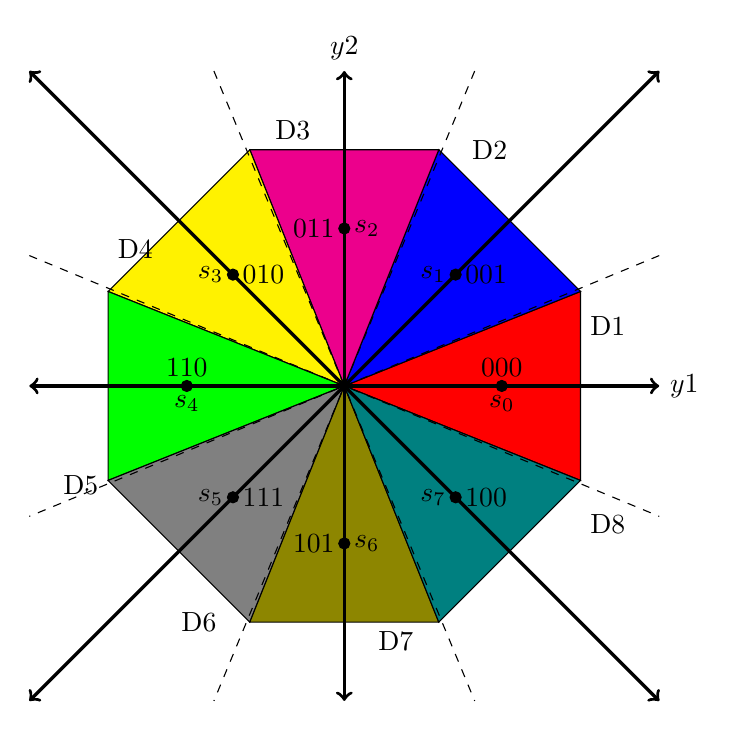
\begin{tikzpicture}
\draw[fill=red]  (0,0) -- (3,1.2) -- (3,-1.2) -- (0,0) -- cycle;
\draw[fill=blue]  (0,0) -- (1.2,3) -- (3,1.2) -- (0,0) -- cycle;
\draw[fill=magenta!100]  (0,0) -- (-1.2,3) -- (1.2,3) -- (0,0) -- cycle;
\draw[fill=yellow]  (0,0) -- (-1.2,3) -- (-3,1.2) -- (0,0) -- cycle;
\draw[fill=green]  (0,0) -- (-3,1.2) -- (-3,-1.2) -- (0,0) -- cycle;
\draw[fill=gray]  (0,0) -- (-3,-1.2) -- (-1.2,-3) -- (0,0) -- cycle;
\draw[fill=olive]  (0,0) -- (-1.2,-3) -- (1.2,-3) -- (0,0) -- cycle;
\draw[fill=teal]  (0,0) -- (1.2,-3) -- (3,-1.2) -- (0,0) -- cycle;
\draw[<->,very thick] (-4,0)--(4,0) node[right]{$y1$};
\draw[<->,very thick] (0,-4)--(0,4) node[above]{$y2$};
\draw[dashed] (4,1.656)--(-4,-1.656);
\draw[dashed] (1.656,4)--(-1.656,-4);
\draw[dashed] (-1.656,4)--(1.656,-4);
\draw[dashed] (-4,1.656)--(4,-1.656);
\draw[<->,very thick](-4,-4)--(4,4);
\draw[<->,very thick](-4,4)--(4,-4);

\filldraw[black] (2,0) circle (2pt) node[below] {$s_0$} node[above] {000};
\filldraw[black] (1.414,1.414) circle (2pt) node[left] {$s_1$} node[right] {001};
\filldraw[black] (0,2) circle (2pt) node[right] {$s_2$} node[left] {011};
\filldraw[black] (-1.414,1.414) circle (2pt) node[left] {$s_3$} node [right] {010};
\filldraw[black] (-2,0) circle (2pt) node[below] {$s_4$} node[above] {110};
\filldraw[black] (-1.414,-1.414) circle (2pt) node[left] {$s_5$} node[right] {111};
\filldraw[black] (0,-2) circle (2pt) node[right] {$s_6$} node[left] {101};
\filldraw[black] (1.414,-1.414) circle (2pt) node[left] {$s_7$} node [right] {100};

\foreach \coordinate/\label/\pos in {{(3,1)/D1/below right},{(1.5,3)/D2/right},{(-1,3)/D3/above right},{(-3,1.5)/D4/above right},{(-3,-1.5)/D5/above left},{(-1.5,-3)/D6/left},{(1,-3)/D7/below left},{(3,-2)/D8/above right}} \node[\pos] at \coordinate {\label};

\end{tikzpicture}
